
 
 \section{Introduction}
 
 Le but de cette partie est de comprendre ce qu'est une molécule, d'un point de vue électronique et nucléaire. Pour la partie électronique, on étudiera les liaisons chimiques entre atomes, principalement sur des molécules très simples, comme $H^+_2$. Pour la partie nucléaire, on va de nouveau séparer le mouvement des noyaux en une partie vibratoire, vue comme un oscillateur harmonique, et une partie rotationnelle, vue comme un rotateur rigide.
 
 \subsection{Ordres de grandeur}
 
 En physique moléculaire, les longueurs caractéristiques seront déterminées par la taille des liaisons chimiques entre les atomes, qui sont de l'ordre de l'$\mathring{A}$ngström, soit $10^{-10}m$.\newline
 En partant de la longueur caractéristique d'une liaison chimique ($\Delta x \sim 1\mathring{A}$) et de la relation d'incertitude d'Heisenberg, on peut déterminer l'énergie caractéristique des liaisons : 
 \begin{equation*}
     \Delta x\times \Delta P \geq \hbar
 \end{equation*}
 \begin{equation*}
     E_{el} \approx \frac{P^2}{2m} \approx \frac{\hbar ^2}{2mx^2} \approx 6.10^{-19}J
 \end{equation*}
  L'ordre de grandeur des énergies en action sera donc de l'ordre de l'électron-volt, voire moins, contrairement à celles utilisées en physique nucléaires, qui dépassent allègrement le $MeV$. C'est pourquoi on utilisera plus volontiers le $cm^{-1}$ comme unité, reliée à l'$eV$ par la relation $E = \frac{\hbar c}{\lambda}$, qui permet de calculer : $1eV = 8065.54 cm^{-1}$.\newline
  Si on représente maintenant une liaison chimique comme un électron oscillant entre deux noyaux à la manière d'un oscillateur harmonique, on peut y associer une fréquence $\omega_{el} = \sqrt{\frac{k}{m}}$.\newline
  De la même manière, on peut associer une fréquence de vibration aux noyaux de la molécule : $\omega_{Nu} = \sqrt{\frac{k}{M}}$.\newline
  Le rapport des énergies de ces deux vibrations sera donc : 
  \begin{equation*}
      \frac{E_{Nu}}{E_{el}} = \frac{\hbar \omega_{Nu}}{\hbar\omega_{el}} = \sqrt{\frac{m}{M}}
  \end{equation*}
  Avec m, la masse de l'électron et M la masse du noyau (M ~ 2000m). On peut donc donner un ordre de grandeur pour l'énergie de vibration des noyaux : 
  \begin{equation*}
      E_{Nu} = \sqrt{\frac{m}{M}}E_{el} \sim 0.01 eV
  \end{equation*}
  Enfin, l'ensemble de la molécule peut avoir un mouvement de rotation sur elle-même dont l'énergie sera : 
  \begin{equation*}
      E_{rot} = \frac{J^2}{2I} \approx \frac{\hbar^2}{Ma^2} = \frac{m}{M}\frac{\hbar^2}{ma^2} = \frac{m}{M}E_{el}
  \end{equation*}
 Cette énergie sera donc de l'ordre du $meV$, et d'autant plus petite que la molécule est grosse.\newline
 Nous avons donc trois types d'excitation moléculaire, associés chacun à un ordre d'énergie, et donc de fréquence et de temps, tels que représentés dans la Figure \ref{fig:niv_excitation_mol}.\newline
 \begin{figure}[ht]
    \centering
    \includegraphics[scale=0.80]{Images3/Types d'excitation moléculaire.PNG}
    \caption{Niveaux d'excitation moléculaire}
    \label{fig:niv_excitation_mol}
\end{figure}
Des énergies supérieures à une dizaine d'$eV$ provoqueront une photoionisation de la molécule.

\section{Hamiltonien}

\subsection{Représentation adiabatique de l'Hamiltonien moléculaire}

Pour résoudre l'Hamiltonien associé à une molécule, on va d'abord le séparer en une partie nucléaire et une partie électronique. Donc avec R les coordonnées des noyaux et r celles des électrons, on aura : 
\begin{equation*}
    H_{mol}(r,R)  \Psi(r,R) = E\Psi(r,R)
\end{equation*}
\begin{equation*}
    H_{mol}(r,R) \to [H_{el}(r,R) + T_{Nu}(R)]\Psi(r,R) = E\Psi(r,R)
\end{equation*}
On peut développer les fonctions propres de l'Hamiltonien global en terme des fonctions propres de $H_{el}$ et $T_{Nu}$, que l'on notera $\psi^{el}_m(r;R)$\footnote{(r;R) signifie que R est fixé et r varie} et $\phi^{Nu}_m(R)$.
\begin{equation*}
    \Psi(r,R) = \sum\limits_m \psi^{el}_m(r;R) \phi^{Nu}_m(R)
\end{equation*}
Avec, bien entendu, les relations : 
\begin{equation*}
    H_{el}\psi^{el}_m(r;R) = E^{el}_m\psi^{el}_m(r;R) \quad \textrm{et} \quad \braket{\psi^{el}_m(r;R)}{\psi^{el}_n(r;R)} = \delta_{mn} 
\end{equation*}
Si on applique l'Hamiltonien, on aura donc :
\begin{equation*}
    T_{Nu} \sum\limits_m \psi^{el}_m \phi^{Nu}_m + H_{el}\sum\limits_m \psi^{el}_m \phi^{Nu}_m  = E\psi^{el}_m\phi^{Nu}_m
\end{equation*}
En multipliant à gauche par $\bra{\psi^{el}_n}$, on obtient :
\begin{equation}\label{eq:1}
    \sum\limits_m \mel{\psi^{el}_n}{T_{Nu}}{\psi^{el}_m \phi^{Nu}_m} + \delta_{mn}E^{el}_m\phi^{Nu}_m = E \delta_{mn}\phi^{Nu}_m
\end{equation}
Sachant que $T_{Nu} = \sum\limits_{\alpha}-\frac{\hbar^2}{2M_{\alpha}}\nabla_{\alpha}^2$, avec $\alpha$ les différents noyaux, la somme de l'équation \ref{eq:1} devient :
\begin{equation}\label{eq:2}
\begin{split}
    \sum\limits_m \mel{\psi^{el}_n}{T_{Nu}}{\psi^{el}_m \phi^{Nu}_m} = & - \frac{\hbar^2}{2}\sum\limits_{\alpha}\frac{1}{M_{\alpha}}\nabla_{\alpha}^2\phi^{Nu}_m\delta_{mn} \\
    & - \hbar^2\sum\limits_{\alpha}\frac{1}{M_{\alpha}}\nabla_{\alpha}\phi^{Nu}_m\nabla_{\alpha}\psi^{el}_m \\
    & - \frac{\hbar^2}{2}\sum\limits_{\alpha}\frac{1}{M_{\alpha}}\nabla_{\alpha}^2\psi^{el}_m\phi^{Nu}_m    
\end{split}
\end{equation}
Dans l'équation \ref{eq:2}, la première ligne correspond à l'Hamiltonien du noyau, la seconde aux interaction entre les noyaux et les électrons, que l'on notera $C_{nm}^{(1)}$, et la troisième aux interactions des électrons entre eux, notée $C_{nm}^{(2)}$.\newline
On remarquera que les termes $C_{ii}^{(1)}$ sont nuls, et que $C_{nm}^{(1)} = - C_{mn}^{(1)}$
L'Hamiltonien moléculaire total en représentation adiabatique ressemblera donc à :
\begin{equation*}
    H_{mol} = 
    \begin{pmatrix}
    T_{Nu} + \epsilon_o^{el} + C_{00}^{(2)} & C_{01}^{(1)}+C_{01}^{(2)} & C_{02}^{(1)}+C_{02}^{(2)} & \cdots \\
    C_{10}^{(1)}+C_{10}^{(2)} & T_{Nu} + \epsilon_1^{el} + C_{11}^{(2)} & C_{12}^{(1)}+C_{12}^{(2)} & \cdots \\
    \vdots  & \vdots  & \vdots & \ddots  \\
    \end{pmatrix}
\end{equation*}
Ou encore : 
\begin{equation*}
    \mel{\psi^{el}_n}{H_{mol}}{\psi^{el}_m} = \delta_{mn}T_{Nu} + \delta_{mn}E_m^{el} + C_{nm}^{(1)} + C_{nm}^{(2)}
\end{equation*}
Partant de cette représentation, on pourra faire deux approximations différentes : \newline
La représentation adiabatique, dans laquelle on va négliger les éléments non-diagonaux, et l'approximation de Born-Oppenheimer, dans laquelle on va négliger tous les $C_{nm}$.\newline
Cette dernière approximation va supprimer complètement la dépendance nucléaire des électrons.\newline
En pratique, en calculant les solutions pour un certain nombre de R différents, on pourra obtenir une hyper-surface d'énergie potentielle sur laquelle les noyaux peuvent se trouver. Elles auront une dimension égale à $3N - 5$ pour une molécule linéaire, et $3N - 6$ pour une molécule non-linéaire. Avec N le nombre d'atomes. Chacune de ces hyper-surfaces auront des sous-niveaux d'énergies correspondant aux états de vibration et de rotation des noyaux.

\subsection{Limites de l'approximation de Born-Oppenheimer}

L'approximation de Born-Oppenheimer peut se résumer à l'équation suivante : 
\begin{equation*}
    [\hat{H}-E_m]\ket{\psi_m} = 0
\end{equation*}
Si on dérive cette expression par rapport aux coordonnées des noyaux, on obtient : 
\begin{equation}\label{eq:3}
    [\hat{H}'-E_m']\ket{\psi_m} + [\hat{H}-E_m]\ket{\psi_m'} = 0
\end{equation}
Que l'on peut multiplier par $\bra{\psi_m}$ : 
\begin{equation*}
\begin{split}
    \mel{\psi_m}{H'}{\psi_m} - \mel{\psi_m}{E_m'}{\psi_m} + \mel{\psi_m}{H}{\psi_m'} + \mel{\psi_m}{E_m}{\psi_m'} & = 0 \\
    \mel{\psi_m}{H'}{\psi_m} - E_m'\braket{\psi_m}{\psi_m} + \braket{H\psi_m}{\psi_m'} - E_m \braket{\psi_m}{\psi_m'} & = 0 \\
    \mel{\psi_m}{H'}{\psi_m} - E_m' + E_m\braket{\psi_m}{\psi_m'} - E_m \braket{\psi_m}{\psi_m'} & = 0 \\
    \mel{\psi_m}{H'}{\psi_m} & = E_m'
    \end{split}
\end{equation*}
Le passage de $\mel{\psi_m}{H}{\psi_m'}$ à $\braket{H\psi_m}{\psi_m'}$ est correct car H est un opérateur auto-adjoint.\newline
Si on reprend l'équation \ref{eq:3} et qu'on la multiplie, cette fois, par $\bra{\psi_m}$, on obtient : 
\begin{equation*}
    \begin{split}
        \mel{\psi_n}{H'}{\psi_m} - \mel{\psi_n}{E_m'}{\psi_m} + \mel{\psi_n}{H}{\psi_m'} + \mel{\psi_n}{E_m}{\psi_m'} & = 0 \\
        \mel{\psi_n}{H'}{\psi_m} - E_m'\braket{\psi_n}{\psi_m} + \braket{H\psi_n}{\psi_m'} - E_m \braket{\psi_n}{\psi_m'} & = 0 \\
        \mel{\psi_n}{H'}{\psi_m} + E_n\braket{\psi_n}{\psi_m'} - E_m \braket{\psi_n}{\psi_m'} & = 0 \\
        \frac{\mel{\psi_n}{H'}{\psi_m}}{E_n-E_m} & = \braket{\psi_n}{\frac{\p\psi_m}{\p R_{\alpha}}}
    \end{split}
\end{equation*}
Le terme de droite de la dernière égalité étant proportionnel à $C_{nm}^{(1)}$, qui a été négligé dans les deux approximations, le terme de gauche doit être très petit dans nos approximations. Or il est inversement proportionnel à $E_n-E_m$, donc lorsque deux états auront des énergies très proches, l'approximation ne tiendra plus.\newline
Ce "problème" arrive ssi 
\begin{equation}\label{eq:4}
    \begin{split}
        & \mel{\psi_1}{H}{\psi_1} = \mel{\psi_2}{H}{\psi_2} \\
        & \mel{\psi_1}{H}{\psi_2} = \mel{\psi_2}{H}{\psi_1} = 0\\
    \end{split}
\end{equation}
Les équations \ref{eq:4} donnent 2 contraintes supplémentaires, sauf dans le cas où $\psi_1$ et $\psi_2$ sont de symétrie différentes, car alors on a toujours : $\mel{\psi_1}{H}{\psi_2} = 0$, et seule la première équation est une contrainte.\newline
La dimension du domaine de croisement sera donc égale à $D-2$ pour des états de même symétrie, et à $D-1$ pour des états de symétries différentes, avec D la dimension des hyper-surfaces d'énergie.\newline

\subsection{Définitions rapides}

On appellera $D_0$ l'énergie de dissociation, déterminée expérimentalement comme la différence d'énergie entre la molécule liée et les atomes entièrement séparés.\newline
On appellera $D_e$ la profondeur du puits de potentiel, la différence entre l'énergie des atomes complètement séparés et le minimum d'énergie possible dans le modèle considéré (ici Born-Oppenheimer).\newline
Ces deux grandeurs sont très proches mais pas égales. Par exemple, dans le cadre de B-O, on ne prend pas en compte la masse des noyaux, donc $H^+_2$ et $D^+_2$ auront la même valeur de $D_e$ mais des $D_0$ différents.\newline
Enfin, on appellera $r_e$ (ou $R_e$), la distance d'équilibre, définie comme la distance pour laquelle le potentiel est minimal.
 \begin{figure}[ht]
    \centering
    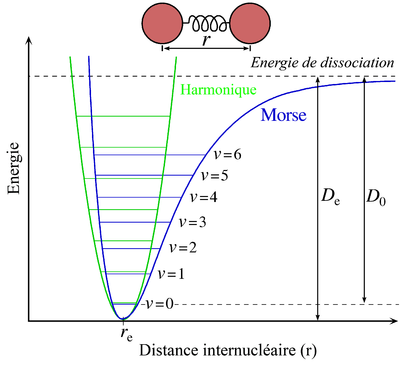
\includegraphics[scale=0.80]{Images3/400px-Morse-potential-fr.png}
    \caption{Illustration de $D_0$ et $D_e$}
\end{figure}

\subsection{Système de coordonnées}

Pour diminuer le nombre de couplages entre les degrés de liberté, on va changer de système de coordonnées.\newline
Par défaut, on utilisait, pour la molécule $H^+_2$, les coordonnées $r_{oi}, R_A, R_B$, avec $r_{oi}$ la position de l'électron et $R_A$ et $R_B$ les positions des deux protons. Le tout par rapport à une origine arbitraire.\newline
 \begin{figure}[ht]
    \centering
    \includegraphics[scale=0.65]{Images3/Coordonnées.png}
    \caption{Coordonnées}
\end{figure}
La première étape consiste à remplacer les coordonnées des noyaux ($R_A$ et $R_B$) par les coordonnées du centre de masse ($R_N$) et les coordonnées du noyau B par rapport au centre de masse (R). R et $R_N$ sont donc définis par :
\begin{equation*}
    \begin{split}
        R &= R_A - R_B \\
        R_N &= \frac{M_AR_A + M_BR_B}{M_A+M_B}
    \end{split}
\end{equation*}
On peut donc réécrire l'Hamiltonien dans ces coordonnées :
\begin{equation*}
    \begin{split}
        \frac{\p}{\p R_A} &=  \frac{\p}{\p R}\frac{\p R}{\p R_A} + \frac{\p}{\p R_N}\frac{\p R_N}{\p R_A} = \frac{\p}{\p R} + \frac{\p}{\p R_N} \\
        \frac{\p}{\p R_B} &= -\frac{\p}{\p R} + \frac{M_B}{M_A+M_B}\frac{\p}{\p R_N} \\
        \nabla^2_{R_A} &= \nabla^2_{R} + 2\frac{M_A}{M_A+M_B}\nabla_{R}\nabla_{R_N} + (\frac{M_A}{M_A+M_B})^2\nabla^2_{R_N} \\
        \nabla^2_{R_B} &= \nabla^2_{R} - 2\frac{M_B}{M_A+M_B}\nabla_{R}\nabla_{R_N} + (\frac{M_B}{M_A+M_B})^2\nabla^2_{R_N} \\
        H &= -\frac{\hbar^2}{2}(\frac{1}{M_A}+\frac{1}{M_B})\nabla^2_{R} - \frac{\hbar^2}{2(M_A+M_B)}\nabla^2_{R_N} - \frac{\hbar^2}{2m}\sum\limits_i \nabla^2_{r_{oi}} +V
    \end{split}
\end{equation*}
La deuxième étape va remplacer les coordonnées du centre de masse des noyaux ($R_N$) par les coordonnées du centre de masse de la molécule complète ($R_{CM}$), et redéfinir les coordonnées des électrons par rapport au centre de masse. On aura donc des coordonnées : {$r_i$, $R$, $R_{CM}$}, avec :
\begin{equation*}
    \begin{split}
        r_i &\equiv r_{oi} - R_N \\
        R_{CM} &\equiv \frac{m\Sigma r_{oi}+(M_A+M_B)R_N}{M}
    \end{split}
\end{equation*}
Avec M la masse totale.\newline
En définissant $\mu$ comme la masse réduite des deux noyaux, on peut une nouvelle fois réécrire l'Hamiltonien :
\begin{equation*}
    \begin{split}
        \pdv{}{x_{oi}} &= \sum\limits_j\pdv{}{x_j}\pdv{x_j}{x_{oi}} + \pdv{}{X_{CM}}\pdv{X_{CM}}{x_{oi}} = \pdv{}{x_i} + \frac{m}{M}\pdv{}{X_{CM}} \\
        \pdv{}{X_N} &= \sum\limits_j\pdv{}{x_j}\pdv{x_j}{X_N} + \pdv{}{X_{CM}}\pdv{X_{CM}}{X_N} = - \sum\limits_j\pdv{}{x_j} + \frac{(M_A + M_B)}{M}\pdv{}{X_{CM}} \\
        \nabla^2_{r_{oi}} &= \nabla^2_{r_{i}} + 2\frac{m}{M}\nabla_{r_i}\nabla_{R_{CM}} + (\frac{m}{M})^2\nabla^2_{R_{CM}} \\
        \nabla^2_{R_N} &= \sum\limits_j\nabla^2_{r_j} + \sum\limits_i\sum\limits_{j\neq i}\nabla_{r_i}\nabla_{r_j} + \frac{(M_A + M_B)^2}{M^2}\nabla^2_{R_{CM}} - 2\frac{(M_A + M_B)}{M}\sum\limits_j \nabla_{r_j}\nabla_{R_{CM}}\\
        H &= -\frac{\hbar^2}{2\mu}\nabla^2_R - \frac{\hbar^2}{2}\frac{(M_A + M_B)}{M^2} + \frac{\hbar^2}{M}\sum\limits_j(\nabla_{r_j}\nabla_{R_{CM}}) \\
        &\quad -\frac{\hbar^2}{2(M_A + M_B)}\sum\limits_i\sum\limits_{j\neq i}(\nabla_{r_j}\nabla_{r_i}) \\
        &\quad -\frac{\hbar^2}{2m}\sum\limits_i \nabla^2_{r_{i}} - \frac{\hbar^2}{M}\sum\limits_i(\nabla_{r_i}\nabla_{R_{CM}}) - \frac{\hbar^2 m}{2M^2}\nabla^2_{R_{CM}} + V(r_i, R) \\
    \end{split}
\end{equation*}

\subsection{Solutions de l'Hamiltonien}\label{Solutions de l'hamiltonien}

Maintenant qu'on a un Hamiltonien dans des coordonnées plus accessibles, on va pouvoir essayer d'en trouver des solutions approchées.\newline
Le terme en $\nabla_{r_j}\nabla_{r_i}$ correspond au déplacement du centre de masse dû au mouvement des électrons. Celui-ci étant considéré comme très faible, on pourra le négliger.\newline
Il nous reste donc : 
\begin{equation*}
    H = -\frac{\hbar^2}{2\mu}\nabla^2_R - \frac{\hbar^2}{2M}\nabla^2_{R_{CM}} -\frac{\hbar^2}{2m}\sum\limits_i \nabla^2_{r_{i}} + V(r_i, R)
\end{equation*}
On peut donc séparer le mouvement du centre de masse et le mouvement interne de la molécule : 
\begin{equation*}
    \Psi = f(R_{CM})\Psi'(R,r_i)
\end{equation*}
Avec f satisfaisant l'équation : 
\begin{equation*}
    \frac{\frac{-\hbar^2}{2M}\nabla^2_{R_{CM}}f}{f} = E_{CM}
\end{equation*}
La solution de cette équation est une onde plane :
\begin{equation*}
    f = e^{i\Vec{K}\Vec{R_{CM}}}
\end{equation*}
Avec
\begin{equation*}
    K^2 = \frac{2E_{CM}M}{\hbar^2}
\end{equation*}
$\Psi'$, quant à lui, doit être solution de l'Hamiltonien interne :
\begin{equation*}
    \left[-\frac{\hbar^2}{2\mu}\nabla^2_R - \frac{\hbar^2}{2m}\sum\limits_i \nabla^2_{r_{i}} + V(r_i, R)\right]\Psi' = (E_T-E_{CM})\Psi'
\end{equation*}
Par la suite, on notera E l'énergie interne ($E = E_T - E_{CM}$).\newline
On peut maintenant appliquer l'approximation de Born-Oppenheimer pour séparer les Hamiltoniens électronique et nucléaire. On aura donc une solution du type : 
\begin{equation*}
    \Psi'(r,R) = \chi^{Nu}_m(R)\psi^{el}_m(r;R)
\end{equation*}
Avec : 
\begin{equation*}
    \left[-\frac{\hbar^2}{2\mu}\nabla^2_R + E^{el}_m(R) - E\right] \chi^{rv}_m(R) = 0
\end{equation*}
Ceci correspond à l'équation de Schrödinger pour une particule dans un champ central à symétrie sphérique. On peut donc séparer $\chi$ en une partie angulaire et une partie radiale : 
\begin{equation*}
    \chi^{Nu}_m(R) = F(R)Y^m_J(\theta\phi)
\end{equation*}
Pour décrire la rotation de la molécule, on va passer en coordonnées sphériques : 
\begin{equation*}
    \Vec{R} \rightarrow (R, \theta, \phi)
\end{equation*}
Dans ces coordonnées, le laplacien s'écrit : 
\begin{equation*}
    \nabla^2_R = \frac{1}{R^2}\pdv{}{R}\left(R^2\pdv{}{R}\right) + \frac{N^2}{\hbar^2R^2}
\end{equation*}
Avec $N^2$ le moment angulaire de rotation définit comme :
\begin{equation*}
    N^2 \equiv -\hbar^2\left[\frac{1}{sin\theta}\pdv{}{\theta}\left(sin\theta\pdv{}{\theta}\right) + \frac{1}{sin^2\theta}\pdv[2]{}{\phi}\right]
\end{equation*}
De valeur propre $N(N+1)$.\newline
On a donc : 
\begin{equation*}
    \left[\frac{-\hbar^2}{2\mu}\frac{1}{R^2}\pdv{}{R}\left(R^2\pdv{}{R}\right) + \frac{N(N+1)\hbar^2}{2\mu R^2} + E^{el}(R)\right]F(R) = EF(R)
\end{equation*}
En posant $G(R) = RF(R)$, on obtient :
\begin{equation*}
    \frac{-\hbar^2}{2\mu}G''(R) + \left[\frac{N(N+1)\hbar^2}{2\mu R^2} + E^{el}(R)\right]G(R) = EG(R)
\end{equation*}
On va maintenant s'intéresser à la composante vibrationnelle du mouvement, donc en considérant que $N = 0$. Pour cela, on va faire le changement de coordonnée suivant : 
\begin{equation*}
    Q = \sqrt{\mu}(R-R_e)
\end{equation*}
Dans le but d'avoir quelque chose qui ressemble à un oscillateur harmonique ($R_e$ est la distance d'équilibre définie plus tôt). L'Hamiltonien s'écrit alors : 
\begin{equation*}
    -\frac{\hbar^2}{2}\psi''_{vib}(Q) + E^{el}(Q)\psi_{vib}(Q) = E_{vib}\psi_{vib}(Q)
\end{equation*}
En $R = R_e$, $Q = 0$, on peut donc faire le développement de Taylor de $E^{el}(Q)$ suivant autour de $R_e$ :
\begin{equation*}
    E^{el}(Q) \approx E^{el}(0) + \left. \dv{E^{el}(Q)}{Q}\right|_{Q = 0}Q + \left. \dv[2]{E^{el}(Q)}{Q}\right|_{Q = 0}Q^2 + \dots
\end{equation*}
En $R = R_e$, on a un minimum pour l'énergie, donc $\dv{E^{el}}{Q} = 0$, et si on considère qu'on se trouve dans l'état fondamental, $E^{el}(0) = 0$ également.\newline
Si on définit maintenant $\lambda = \omega^2 \equiv \left. \dv[2]{E^{el}(Q)}{Q}\right|_{Q = 0} $, on a donc un potentiel harmonique et l'Hamiltonien devient :
\begin{align*}
    H_{vib} &= -\frac{\hbar^2}{2}\dv[2]{}{Q} +\lambda Q^2\\
    H_{vib} &= \frac{1}{2}(P^2_Q + \lambda Q^2)
\end{align*}
(Avec $P_Q$ l'impulsion par rapport à Q).\newline
Les valeurs propres de cet Hamiltonien donnent les énergies des niveaux de vibration (v) :
\begin{equation*}
    E_v = (v + \frac{1}{2})h\nu
\end{equation*}
Et les fonctions propres sont : 
\begin{equation*}
    \psi_v(Q) = \left[(\frac{\gamma}{\pi})^{\frac{1}{2}}\frac{1}{2^v(v!)} \right]^{\frac{1}{2}}e^{\frac{1}{2}\gamma Q^2}H_v(\gamma^{\frac{1}{2}}Q)
\end{equation*}
Avec $\gamma \equiv \frac{2\pi \nu}{\hbar}$, et $H_v(x)$ les polynômes d'Hermite, dont les 4 premiers termes sont : 
\begin{equation*}
    \begin{split}
        H_0(x) &= 1\\
        H_1(x) &= 2x\\
        H_2(x) &= 4x^2-2\\
        H_3(x) &= 8x^3-6x        
    \end{split}
\end{equation*}
Si on fait maintenant l'approximation du rotateur rigide, à savoir $R\approx R_e$, on obtient une expression pour l'énergie composée de 3 termes : 
\begin{equation*}
    E = E^{el}(R_e) + \hbar\omega(v+\frac{1}{2}) + \frac{N(N+1)\hbar^2}{2\mu R_e^2}
\end{equation*}
Le premier est l'énergie de liaison électronique, le deuxième est l'énergie de vibration des noyaux, et le troisième l'énergie de rotation du système. On peut simplifier le dernier terme en définissant $B \equiv \frac{\hbar^2}{2\mu R_e^2}$, la constante de rotation en Joules, qu'on peut diviser par $hc$ pour l'exprimer en $cm^{-1}$.\newline
On peut donc remarquer qu'avec ces deux approximations (rotateur rigide et oscillateur harmonique) l'Hamiltonien est complètement séparable, l'énergie est la somme des énergies de chaque contribution, et la fonction d'onde est le produit des fonctions associées à ces mêmes contributions : 
\begin{equation*}
    \psi(r,Q,\theta,\phi) = \psi^{el}(r;R)\psi_{vib}(Q)\psi_{rot}(\theta,\phi)
\end{equation*}

\subsection{Potentiel de Morse}

L'approximation harmonique n'est malheureusement proche de la réalité que pour les premiers niveaux d'énergie. Elle devient vite complètement incorrecte pour les niveaux plus élevés, et la dissociation de la molécule ne se fait jamais. Pour améliorer cela, on peut utiliser d'autres formulations de la fonction $E^{el}(R)$, dont la plus connue est celle de M. Morse : 
\begin{equation*}
    E^{el}(R) = D_e(1-e^{-\beta(R-R_e)})^2
\end{equation*}

\begin{figure}[ht]\label{fig:Morse}
    \centering
    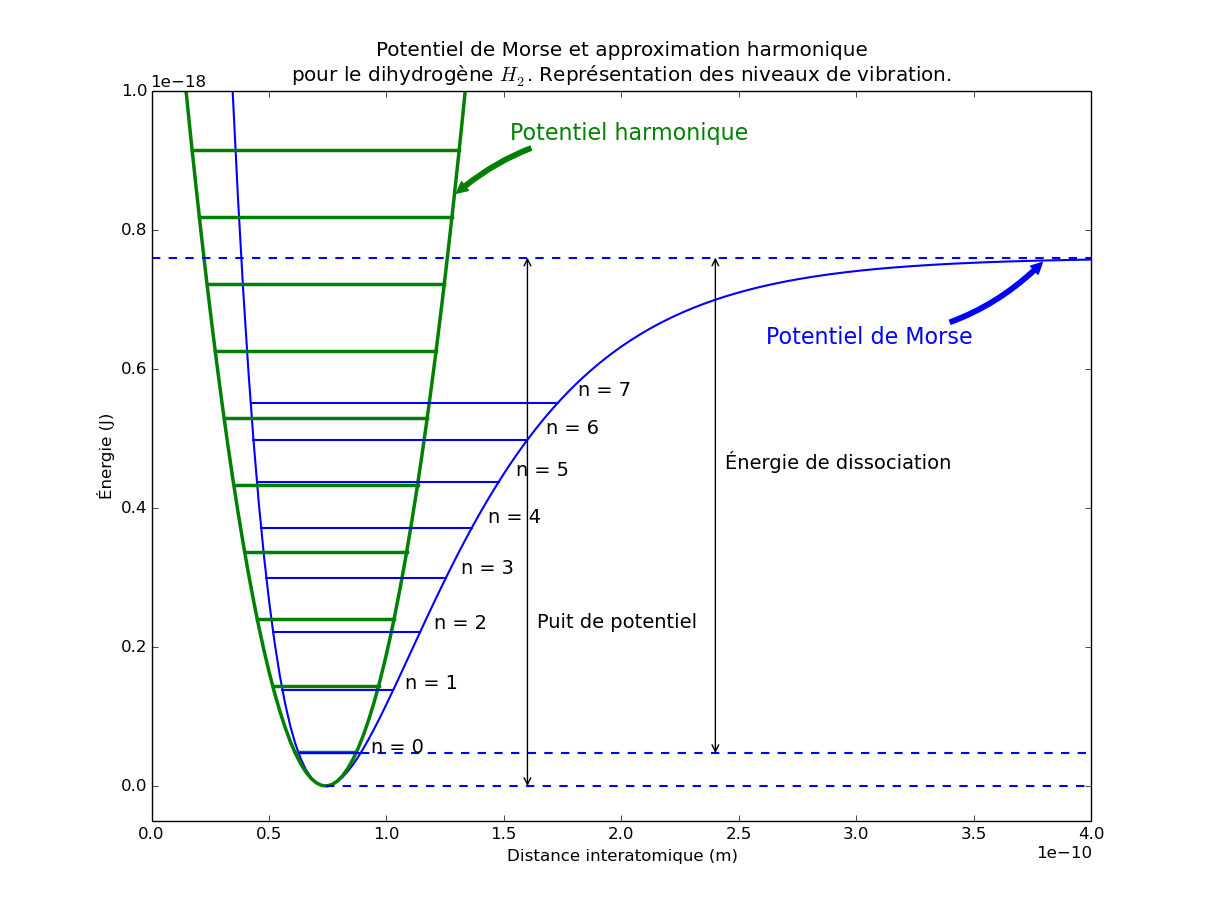
\includegraphics[scale=0.45]{Images3/potentiel_morse-04.png}
    \caption{Comparaison du potentiel harmonique avec le potentiel de morse}
\end{figure}

Ce potentiel est représenté sur la figure \ref{fig:Morse}.
On peut voir que contrairement au potentiel harmonique, celui-ci permet une dissociation de la molécule lorsque la distance entre les noyaux augmente, et elle résout le problème des niveaux d'énergie équidistants du potentiel harmonique.\newline
L'Hamiltonien avec ce nouveau potentiel peut être résolu, et on obtient : 
\begin{equation*}
    \frac{E_{v,J}}{hc} = \omega_e(v+\frac{1}{2})-x_e\omega_e(v+\frac{1}{2})^2+B_eJ(J+1)-DJ^2(J+1)^2-\alpha_e(v+\frac{1}{2})J(J+1)
\end{equation*}
Dans cette expression les paramètres sont en $cm^{-1}$ et se définissent par rapport
aux paramètres du potentiel de Morse :
\begin{equation*}
    \begin{split}
        \omega_e &\equiv \frac{\beta}{2\pi c}\sqrt{\frac{2D_e}{\mu}}\\
        x_e &\equiv \frac{hc\omega_e}{4D_e}\\
        B_e &\equiv \frac{\hbar}{4\pi\mu R_e^2c}\\
        D &\equiv \frac{\hbar^3}{16\pi^3\mu^3\omega_e^2R_e^6c^3} = \frac{4B_e^3}{\omega_e^2}\\
        \alpha_e &\equiv \frac{3\hbar^2\omega_e}{4\mu R_e^2D_e}\left(\frac{1}{aR_e}-\frac{1}{a^2R_e^2}\right) = 6\sqrt{\frac{x_eB_e^3}{\omega_e}}-6\frac{B_e^2}{\omega_e}
    \end{split}
\end{equation*}
La constante de rotation définie précédemment peut s'exprimer comme : 
\begin{equation*}
    B_v = B_e -\alpha_e(v+\frac{1}{2})
\end{equation*}
On peut voir aussi que, dans le cadre de ce modèle, 
\begin{equation*}
    \begin{split}
        D_e &= E(R_e)-E(R=\infty)\\
        D_0 &= E(v=0)-E(R=\infty)
    \end{split}
\end{equation*}
\begin{figure}[ht]
    \centering
    \includegraphics[scale=1.2]{Images3/Niveaux d'énergie Morse.PNG}
    \caption{Fonctions d’onde vibrationnelle pour v= 0, 1, 2 associées au potentiel
électronique de la molécule HF. Ces fonctions d’ondes ont été obtenues par une
approche variationnelle dans une base de sinus en considérant N = J = 0.}
    \label{fig:Niv}
\end{figure}

\section{$H_2^+$ et la liaison chimique}

Pour tester les modèles et développements, on va étudier le système le plus simple, à savoir l'ion $H_2^+$. Celui-ci ne contient qu'un électron et 2 protons, il n'y a donc pas d'interaction électron-électron. Dans le cadre de l'approximation de Born-Oppenheimer, on a l'Hamiltonien suivant : 
\begin{equation*}
    H_{el} = -\frac{\hbar^2}{2m}\nabla^2_i-\frac{Z_Ae^2}{4\pi \epsilon_0||r_i - R_A||}-\frac{Z_Be^2}{4\pi \epsilon_0||r_i - R_B||} +\frac{Z_AZ_B}{4\pi\epsilon_0R}
\end{equation*}
Que l'on peut réécrire en coordonnées confocales $(\mu, \nu, \phi)$, avec :
\begin{equation*}
    \begin{split}
        \mu &= \frac{r_a + r_b}{R}\\
        \nu &= \frac{r_a-r_b}{R}
    \end{split}
\end{equation*}
\begin{equation*}
    H_{el} = -\frac{\hbar^2}{2m_eR^2}\frac{4}{\mu^2-\nu^2}\left[\pdv{}{\mu}(\mu^2-1)\pdv{}{\mu}+\pdv{}{\nu}(1-\nu^2)\pdv{}{\nu}+\left(\frac{1}{\mu^2-1}+\frac{1}{1-\nu^2}\right)\pdv[2]{}{\phi}\right] - \frac{2e^2}{R}\left(\frac{1}{\nu + \mu}+\frac{1}{\mu-\nu}\right) + \frac{e^2}{R} 
\end{equation*}
Les solutions de cet Hamiltonien seront de la forme : 
\begin{equation*}
    \psi(\mu,\nu,\phi) = F(\mu,\nu)e^{im\phi}
\end{equation*}
Avec
\begin{equation*}
    F(\mu,\nu) = M(\mu)N(\nu)
\end{equation*}
Nous avons donc bien $\pdv[2]{\psi}{\phi} = -m^2\psi$, et M et N satisfont les équations : 
\begin{equation*}
    \begin{split}
        \frac{d}{d\mu}(\mu^2-1)\dv{M}{\mu} + \left(E\mu^2\frac{m_eR^2}{2\hbar^2}+\frac{2}{a_0}\mu R+K-\frac{m^2}{\mu^2-1}\right)M &= 0\\
        \frac{d}{d\nu}(1-\nu^2)\dv{N}{\nu} + \left(E\nu^2\frac{m_eR^2}{2\hbar^2}-K-\frac{m^2}{1-\nu^2}\right)N &= 0
    \end{split}
\end{equation*}
L'équation satisfaite par $\psi(\mu,\nu,\phi)$ pouvant être séparée en une partie dépendante de $\mu$ à gauche et une partie dépendante de $\nu$ à droite de l'égalité, chaque partie est une constante par rapport à l'autre variable, que l'on appelle K, et qui intervient dans les équations pour M et N ci-dessus.\newline
Tout ceci peut être résolu exactement numériquement, et on arrive à le conclusion que les valeurs propres de l'Hamiltonien sont dégénérées en m, et qu'il commute avec l'opérateur $L_z$, car on a une symétrie cylindrique autour de l'axe entre les noyaux. \newline
On va maintenant pouvoir utiliser ces résultats pour tester des modèles.

\subsection{Modèle LCAO, cas général}

Ce modèle consiste à considérer une orbitale moléculaire comme une combinaison linéaire d’orbitales atomiques (Linear Combination of Atomic Orbital). La fonction d'onde moléculaire s'écrit donc :
\begin{equation*}
    \Psi = \sum\limits_i c_i\ket{\phi_i}
\end{equation*}
Où $\Psi$ est une fonction d'onde électronique moléculaire et $\phi$ est une fonction d'onde électronique atomique.\newline
Si on considère seulement 2 fonctions d'onde atomique, on a :
\begin{equation*}
    \begin{split}
        H\Psi &= E\Psi\\
        Hc_1\ket{\phi_1} + Hc_2\ket{\phi_2}  &= E(c_1\ket{\phi_1} + c_2\ket{\phi_2})
    \end{split}
\end{equation*}
Si on multiplie à gauche par $\ket{\phi_1}$ et $\ket{\phi_2}$, on obtient les deux équations suivantes : 
\begin{equation*}
    \begin{split}
        c_1H_{11} + c_2H_{12} &= E(c_1+c_2S_{12})\\
        c_1H_{21} + c_2H_{22} &= E(c_1S_{21}+c_2)
    \end{split}
\end{equation*}
Où $H_{ij} = \mel{\phi_i}{H}{\phi_j}$ et $S_{ij} = \braket{\phi_1}{\phi_2}$. $S_{ij} = S_{ji}$ et représente le recouvrement des orbitales atomiques.\newline
On a donc le système suivant :
\begin{equation*}
    \begin{split}
        (H_{11} - E)c_1 + (H_{12} - ES_{12})c_2 &= 0\\
        (H_{21} - ES_{12})c_1 + (H_{22} - E)c_2 &= 0\\
    \end{split}
\end{equation*}
Représenté sous forme matricielle comme suit :
\begin{equation*}
    \begin{pmatrix}
    H_{11}-E && H_{12}-ES_{12}\\
    H_{21}-ES_{12} && H_{22}-E
    \end{pmatrix}
    \begin{pmatrix}
    c_1\\
    c_2
    \end{pmatrix}
    = 
    \begin{pmatrix}
    0\\
    0
    \end{pmatrix}
\end{equation*}
Si on considère une molécule $H_2$, avec $\phi_1$ et $\phi_2$ les orbitales 1s des deux atomes, alors $H_{11} = H_{22}$, et $H_{12} = H_{21}$, et on trouve :
\begin{equation*}
    \begin{split}
        (H_{11}-E)^2 - (H_{12}-ES_{12})^2 &= 0\\
        [(H_{11}-E) - (H_{12}-ES_{12})][(H_{11}-E) + (H_{12}-ES_{12})] &= 0
    \end{split}
\end{equation*}
Qui donnent deux racines : 
\begin{equation}
    \begin{split}
        E_g &= \frac{H_{11}+H_{12}}{1+S_{12}}\\
        &\quad\quad\textrm{et}\\
        E_u &=\frac{H_{11}-H_{12}}{1-S_{12}}
    \end{split}
\end{equation}

\subsection{Modèle LCAO dans le cas de $H_2^+$}

Dans le cas de $H_2^+$, ne comportant qu'un électron, on a :
\begin{equation*}
    \begin{split}
        H_{11} &= \mel{1s_A}{-\nabla_r-\frac{1}{r_a}}{1s_A} - \mel{1s_A}{\frac{1}{r_b}}{1s_A} + \mel{1s_A}{\frac{1}{R}}{1s_A}\\
        H_{11} &= E_{1s}-\epsilon_{1s}+\frac{1}{R}S
    \end{split}
\end{equation*}
et
\begin{equation*}
    \begin{split}
        H_{12} &= \mel{1s_A}{-\nabla_r-\frac{1}{r_b}}{1s_B} - \mel{1s_A}{\frac{1}{r_b}}{1s_B} + \mel{1s_A}{\frac{1}{R}}{1s_B}\\
        H_{12} &= E_{1s}S-\beta_{1s} + \frac{1}{R}S
    \end{split}
\end{equation*}
Où le terme $\beta$ est une intégrale d'échange sans équivalent classique.\newline
Ces différentes intégrales peuvent être évaluées, et on obtient :
\begin{equation*}
    \begin{split}
        S(R) &= (1+R+\frac{1}{3}R^2)e^{-R}\\
        \epsilon_{1s} &= \frac{1}{R}[1-(1+R)e^{-2R}]\\
        \beta_{1s} &= (1+R)e^{-R}
    \end{split}
\end{equation*}
On a alors les valeurs propres suivantes : 
\begin{equation*}
    E = \frac{H_{11} \pm H_{12}}{1\pm S} = E_{1s} - \frac{\epsilon_{1s}\pm\beta_{1s}}{1\pm S} +\frac{1}{R}
\end{equation*}
Dans le cadre de ce modèle, la stabilité de la liaison provient du terme central (en $\epsilon\pm\beta$), qui est un terme de recouvrement et d'échange sans équivalent classique.\newline
\begin{figure}[ht]
    \centering
    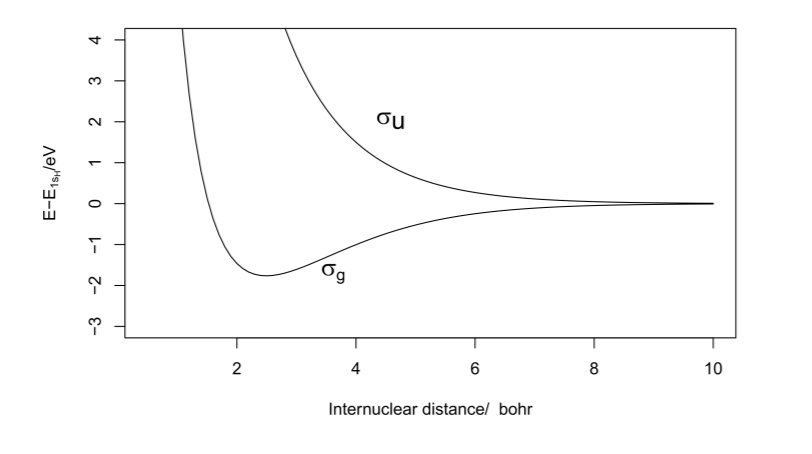
\includegraphics[scale = 0.8]{Images3/LCAOHamiltonien.PNG}
    \caption{Représentation des énergies électroniques solutions de l’Hamiltonien
électronique où on a soustrait la valeur de l’orbitale 1s de l’Hydrogène.}
    \label{fig:Ham}
\end{figure}
\newline
A ces valeurs propres sont associés deux vecteurs propres :
\begin{equation*}
\begin{split}
    \Psi_u &= \frac{1}{\sqrt{2-2S}}[1s_A(r)-1s_B(r)]\\
    \Psi_g &= \frac{1}{\sqrt{2+2S}}[1s_A(r)+1s_B(r)]\\   
\end{split}
\end{equation*}
Ces valeurs et vecteurs propres sont représentés sur les figures \ref{fig:Ham} et \ref{fig:Amp}.\newline
\begin{figure}[ht]
    \centering
    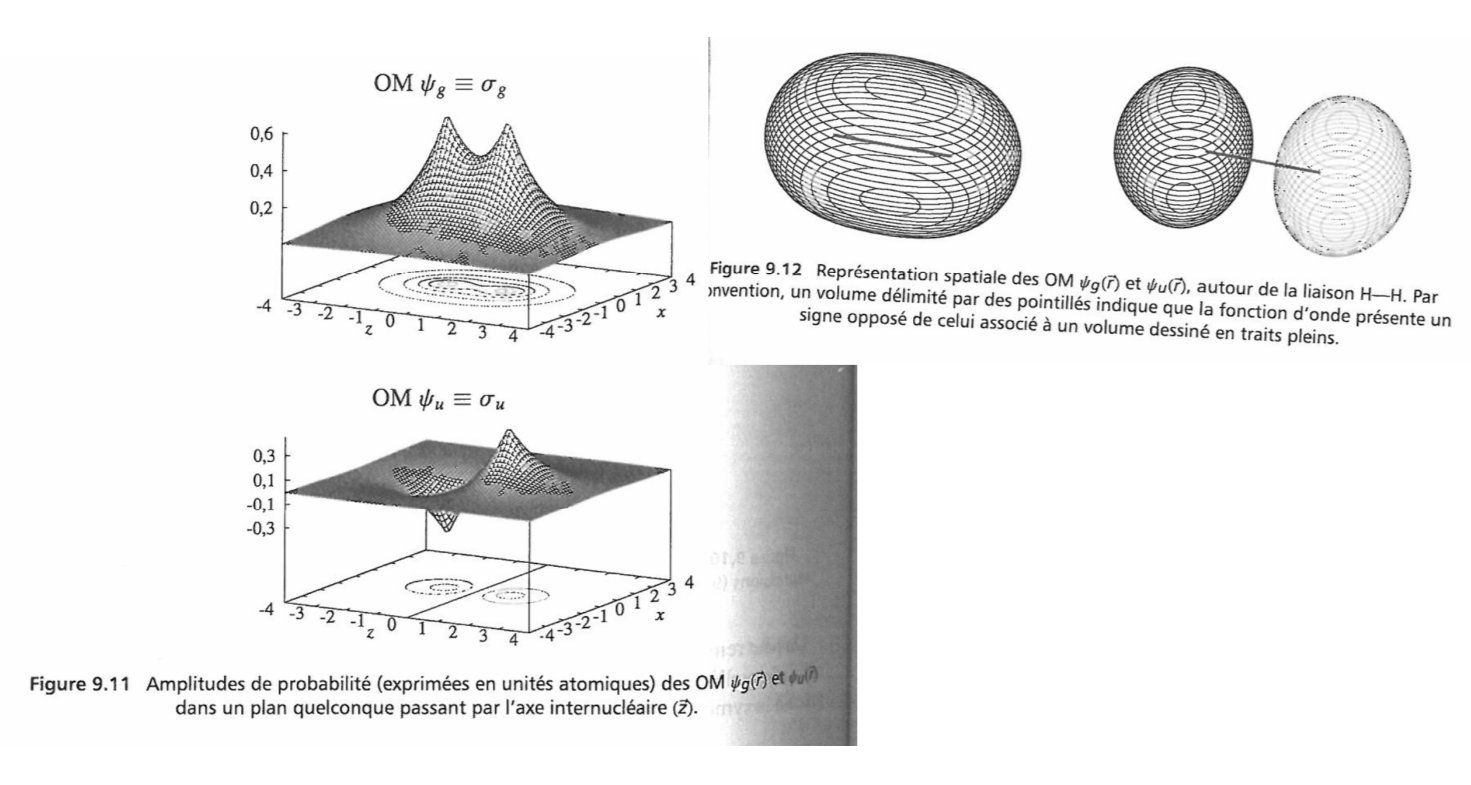
\includegraphics[scale = 0.65]{Images3/LCAOAmplitudes.PNG}
    \caption{Représentation des amplitudes de probabilités des orbitales
moléculaires de $H_2^+$}
    \label{fig:Amp}
\end{figure}
Le détail du calcul des intégrales se trouve dans le sylla fournis par C. Lauzin, mais je crois pas que ce soit matière d'examen, et j'ai la flemme de les retaper.

\subsection{Précision du modèle}

Ce modèle donne, pour $H_2^+$, une valeur $D_e = 1.76eV$ et une distance d'équilibre $R_e = 1.32 \angstrom$. La solution exacte de l'Hamiltonien donne les valeurs : $D_e = 2.78eV$ et $R_e=1.06\angstrom$. Les différences sont donc importantes, mais ce modèle à le mérite d'être très simple et de permettre d'avoir une idées de ce qu'il se passe physiquement. \newline
On peut l'améliorer en utilisant le principe variationnel pour insérer un paramètre dans la fonction d'onde électronique : 
\begin{equation*}
    \Psi_g(r;R) = \frac{1}{\sqrt{2+2S}}\frac{1}{\sqrt{\pi}}\left(\frac{\lambda}{a_0}\right)^{3/2}\left[e^{-\lambda\frac{r_A}{a_0}} + e^{-\lambda\frac{r_B}{a_0}}\right]
\end{equation*}
En minimisant l'énergie électronique par rapport à $\lambda$, on trouve, pour $\lambda = 1.24$ les valeurs $D_e = 2.35eV$ et $R_e = 1.06\angstrom$. Ces valeurs sont déjà beaucoup plus proches de la réalité. Cette amélioration tient mieux compte de l'attraction de l'électron par les deux noyaux simultanément, c'est pourquoi on obtient de meilleurs résultats.\newline
Ces résultats sont cependant loin d'être optimaux, et on peut encore les améliorer de deux manières.\newline
\begin{figure}[ht]
    \centering
    \includegraphics[scale=0.65]{Images3/symétrie.PNG}
    \caption{Utilisation de la symétrie pour ajouter des fonctions d'ondes orbitales}
    \label{fig:sym}
\end{figure}
La première est de permettre aux fonctions d'ondes atomiques de se polariser selon l'axe de la molécule (z) en ajoutant un second paramètre $\eta$ : 
\begin{equation*}
    \phi_A = e^{-\lambda r_A/a_0}(1+\eta z)
\end{equation*}
La seconde est d'augmenter le nombre de fonctions d'ondes atomiques en ajoutant les orbitales excitées. On aura alors : 
\begin{equation*}
    \Psi_g = c_{1s}(1s_A+1s_B) + c_{2s}(2s_A+2s_B) + c_{2p_z}(2p_{z_A}-2p_{z_B}) + \dots
\end{equation*}
L'indice g signifie \textit{gerade}, paire en allemand. On utilise donc les termes de valeur propre +1 de l'opérateur inversion I, tel qu'expliqué dans la figure \ref{fig:sym}.
On pourrait faire la même chose avec les valeurs propres -1 ou $m_l$, qui est nulle pour les orbitales s et $p_z$.\newline

\subsection{de $H_2^+$ à $H_2$}

En passant de 1 à 2 électrons, l'Hamiltonien dans les coordonnées de la figure \ref{fig:Coor} devient : 
\begin{equation*}
    H = -\frac{\hbar^2}{2m}(\nabla^2_1+\nabla^2_2) + \frac{e^2}{4\pi\epsilon_0}\left(-\frac{1}{r_{A1}}-\frac{1}{r_{A2}}-\frac{1}{r_{B1}}-\frac{1}{r_{B2}}+\frac{1}{r_{12}}+\frac{1}{R}\right)
\end{equation*}
Que l'on peut décomposer en\footnote{Attention au signe de $\frac{1}{R}$ qui change car on le considère dans la définition des deux Hamiltoniens monoélectroniques.} : 
\begin{equation*}
    H = H_1 + H_2 +\frac{e^2}{4\pi\epsilon_0}\left(\frac{1}{r_{12}}-\frac{1}{R}\right) \quad \textrm{où} \quad H_i = -\frac{\hbar^2}{2m}\nabla^2_i - \frac{e^2}{4\pi\epsilon_0}\left(\frac{1}{r_{Ai}}+\frac{1}{r_{Bi}}+\frac{1}{R}\right)
\end{equation*}
On peut donc calculer la valeur de l'énergie pour cet Hamiltonien : 
\begin{equation*}
    \langle E \rangle = \mel{\phi}{H}{\phi} = \mel{\phi}{H_1}{\phi} + \mel{\phi}{H_2}{\phi} + \frac{e^2}{4\pi\epsilon_0}\mel{\phi}{\frac{1}{r_{12}}-\frac{1}{R}}{\phi}
\end{equation*}
\begin{figure}[ht]
    \centering
    \includegraphics[scale=0.4]{Images3/Coordonnées2.png}
    \caption{Système de coordonnées utilisé}
    \label{fig:Coor}
\end{figure}
Comme les électrons sont des fermions, ils doivent satisfaire le principe de Pauli, donc la fonction d'onde électronique doit être antisymétrique par rapport à la permutation des deux électrons. Donc $P_{12}\Psi_{elec} = -\Psi_{elec}$, avec $P_{12}$ l'opérateur de permutation des deux électrons.\newline
Le produit de deux fonctions d'ondes de même type (par exemple $g$) doit donc être symétrique par rapport à la permutation des électrons. Si on calcule le produit de 2 orbitales $\sigma_g$ pour les électrons 1 et 2 telles que définies pour $H^+_2$, on obtient : 
\begin{equation*}
    \begin{split}
        \sigma_g(1)\sigma_g(2) &= \frac{1}{\sqrt{2+2S}}[1s_A(1)+1s_B(1)] \frac{1}{\sqrt{2+2S}}[1s_A(2)+1s_B(2)]\\
        \sigma_g(1)\sigma_g(2) &= Cste(1s_A(1)1s_A(2)+1s_A(1)1s_B(2)+1s_B(1)1s_A(2)+1s_B(1)1s_B(2))
    \end{split}
\end{equation*}
Cette expression est bien symétrique par rapport à la permutation des électrons.\newline
On va définir des composantes de spin "up" et "down" pour des valeurs propres de $s_z$ de +1/2 ou -1/2 respectivement : 
\begin{equation*}
    \begin{split}
        \mel{\alpha(1)}{s_z}{\alpha(1)} &= \frac{\hbar}{2}\\
        \mel{\beta}{s_z}{\beta(1)} &= -\frac{\hbar}{2}
    \end{split}
\end{equation*}
Et on notera $\sigma_g(1)\alpha(1) = \sigma_g(1)$ et $\sigma_g(1)\beta(1) = \overline{\sigma_g(1)}$.\newline
On peut maintenant construire un déterminant de Slatter qui va nous permettre de trouver une orbitale moléculaire qui satisfait toutes les propriétés physiques nécessaires : 
\begin{equation*}
    \begin{split}
        \phi(1,2) &= \frac{1}{\sqrt{2}}
        \begin{vmatrix}
            \sigma_g(1)\alpha(1) && \sigma_g(1)\beta(1)\\
            \sigma_g(2)\alpha(2) && \sigma_g(2)\beta(2)
        \end{vmatrix}\\
        \phi(1,2) &= \frac{1}{\sqrt{2}}\sigma_g(1)\sigma_g(2)[\alpha(1)\beta(2)-\beta(1)\alpha(2)]
    \end{split}
\end{equation*}
Cette fonction d'onde est bien antisymétrique par rapport à la permutation des électrons.\newline
On peut maintenant introduire ce $\phi$ dans la valeur de l'énergie trouvée précédemment, et on obtient : 
\begin{equation*}
    E(R) = E(R)_{H^+_2} + \frac{e^2}{4\pi\epsilon_0a_0}\left[\frac{5}{16}-\frac{a_0}{2R}-\frac{a_0}{2R}\left(1+\frac{11R}{8a_0}+\frac{3R^2}{4a_0^2}+\frac{R^3}{6a_0^3}\right)^{\frac{2R}{a_0}}\right]
\end{equation*}
Avec $a_0$ le rayon de Bohr de l'atome d'Hydrogène. On peut maintenant vérifier ce modèle en calculant $D_e$ et $R_e$ : 
\begin{equation*}
    D_e = -2.7eV \quad \quad R_e = 0.85\angstrom
\end{equation*}
Alors que les valeurs trouvées expérimentalement sont :
\begin{equation*}
    D_e = -4.747eV \quad \quad R_e = 0.741\angstrom
\end{equation*}
Visiblement ce modèle n'est pas totalement fiable, on a presque un facteur 2 entre les valeurs théoriques et expérimentales de $D_e$. Ceci vient du fait que $H_2$ peut se dissocier de deux manière différentes, qu'on appellera limite ionique ($H^+ + H^-$) et limite covalente ($H+H$). Ces deux limites interviennent dans l'expression : 
\begin{equation*}
    \sigma_g(1)\sigma_g(2) = \frac{1}{2+2S}(1s_A(1)1s_A(2)+1s_A(1)1s_B(2)+1s_B(1)1s_A(2)+1s_B(1)1s_B(2))
\end{equation*}
En effet, le terme $1s_A(1)1s_A(2)+1s_B(1)1s_B(2)$ correspond à deux électrons centrés sur un des deux noyaux, ce qui donnera la limite ionique, alors que $1s_A(1)1s_B(2)+1s_B(1)1s_A(2)$ correspond à des électrons partagés sur les deux noyaux, ce qui donnera la limite covalente.\newline
Dans notre modèle, ces deux limites ont le même poids, la liaison entre les deux atomes d'hydrogène est donc autant covalente qu'ionique. En réalité, ceci n'est pas forcément vrai, on peut donc essayer d'améliorer le modèle en ajoutant un terme de pondération $\eta$ pour la limite ionique :
\begin{equation*}
    \sigma_g(1)\sigma_g(2) = \frac{1}{2+2S}[\eta(1s_A(1)1s_A(2)+1s_B(1)1s_B(2)) + (1s_A(1)1s_B(2)+1s_B(1)1s_A(2))]
\end{equation*}
En minimisant maintenant l'énergie par rapport à ce nouveau paramètre, on obtient :
\begin{equation*}
    D_e = -4.02eV \quad \quad R_e = 0.75\angstrom
\end{equation*}
Ce qui se rapproche déjà beaucoup plus de la bonne solution, et en ajoutant d'autres fonctions de base, sous la forme : 
\begin{equation*}
    \phi(1,2) = \sum\limits_{i=1}^kc_i\phi_i(1)\phi_i(2)
\end{equation*}
Kolos et Roothan ont réussi à obtenir :
\begin{equation*}
    D_e = -4.746eV \quad \quad R_e = 0.741\angstrom
\end{equation*}
Pour k = 50.

\subsection{ECOC de l'Hamiltonien électronique et symétrie de $\Psi_{electronique}$}

Rappel de MQ :
\begin{itemize}
    \item Les valeurs propres d'un opérateur hermitique ou auto-adjoint ($A\dagger_{mn} = A^*_{nm} = A_{mn}$) sont réelles.
    \item Si deux opérateurs hermitiques commutent, on peut construire une base orthonormée avec leurs vecteurs propres communs.
\end{itemize}
On peut essayer de construire un ECOC (ensemble complet d'opérateurs qui commutent) avec H.\newline
On sait déjà que H commute avec $L_z$. Comme $m_l$ est dégénérée, on va définir un nombre quantique $\lambda = \abs{m_l}$. On utilisera toujours des lettres grecques minuscules pour les valeurs de $m_l$ associées à un seul électron, et des majuscules pour $M_l$, la somme des $m_l$. Ces lettres suivent l'ordre suivant : \newline
Pour 0, on a $\sigma \rightarrow\Sigma$, 1 $\pi\rightarrow\Pi$, 2 $\delta\rightarrow\Delta$, 3 $\phi\rightarrow\Phi$, etc.\newline
Pour une molécule diatomique mononucléaire comme $H_2^+$, l'Hamiltonien commute également avec I, l'opérateur d'inversion des indices des noyaux, dont les valeurs propres sont +1 et -1, notées \textit{g} et \textit{u} pour gerade et ungerade.\newline
L'Hamiltonien commute également avec toutes les opérations de réflexions dont le plan comprend l'axe de la molécule (z). Cette opération est notée $\sigma_v$.Par contre, ce dernier opérateur ne commute pas avec $L_z$. En effet, si on prend par exemple le plan de réflexion tel que $x\rightarrow-x$, sachant que $L_z = -i\hbar(x\pdv{}{y}-y\pdv{}{x})$, on voit bien que ça ne commute pas.\newline
On pourra également remarque que l'opérateur $\sigma_v$ à comme effet, sur une fonction électronique, de changer le signe de $m_l$ (voir figure \ref{fig:sigma_v}). Du coup, dans l'état $\Sigma$, $L_z$ et $\sigma_v$ commutent, et on peut créer un ECOC=[H, $L_z$, I, $\sigma_v$, $S^2$, $S_z$]. Pour les autres états, on aura deux ECOC différents : [H, $L_z$, I, $S^2$, $S_z$] ou [H, I, $\sigma_v$, $S^2$, $S_z$].\newline
\begin{figure}[tpb]
    \centering
    \includegraphics[scale=0.6]{Images3/Complément sigma_v.PNG}
    \caption{Illustration de l’opération $\sigma_v$ sur les coordonnées d’un électron. Cette figure illustre également comment $\sigma_v$ modifie la valeur de $m_l$ de la fonction d’onde électronique.}
    \label{fig:sigma_v}
\end{figure}
L'utilisation de la symétrie simplifie les problèmes de physique moléculaire : 
\begin{equation*}
    I\ket{1s_A} = \ket{1s_B} \Rightarrow \ket{1s_A} \textrm{ n'est pas fonction propre de H}
\end{equation*}
Par contre une combinaison de $\ket{1s_A}$ et $\ket{1s_B}$ oui :
\begin{equation*}
\begin{split}
    I\Psi &= I[C_A\ket{1s_A} + C_B\ket{1s_B}]\\
    &= C_A\ket{1s_B} + C_B\ket{1s_A}
\end{split}
\end{equation*}
Comme les valeurs propres de I sont $\pm 1$, la combinaison sera une fonction propre pour $C_A = \pm C_B$.\newline
Les termes moléculaires seront donc décrits par les valeurs propres de chaque opérateur, tel que représenté sur la figure \ref{fig:notation}.\newline
\begin{figure}
    \centering
    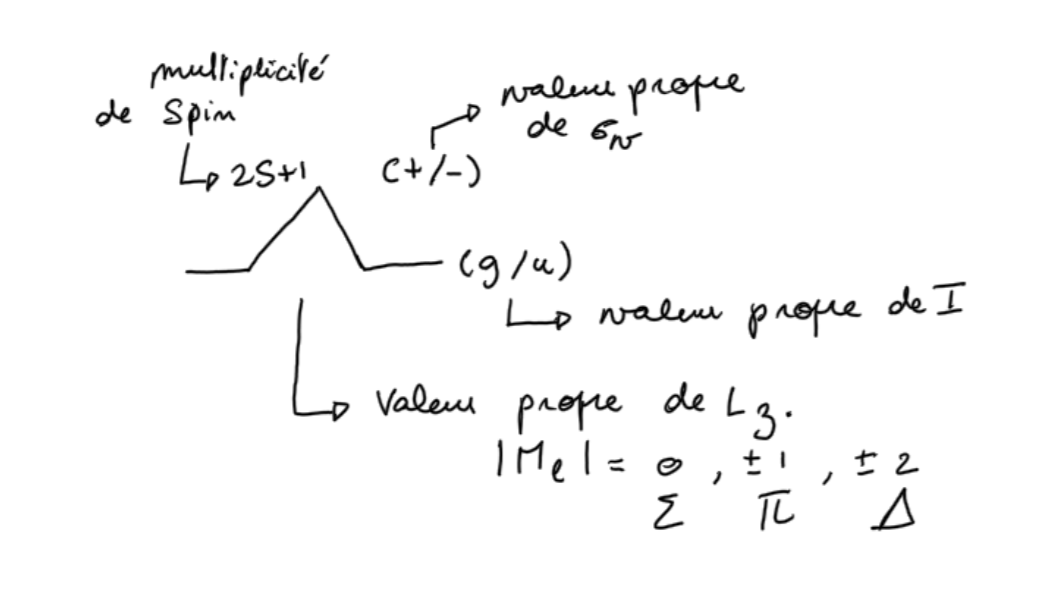
\includegraphics[scale=0.6]{Images3/Notation_mol.PNG}
    \caption{Notation des termes moléculaires}
    \label{fig:notation}
\end{figure}
Les termes sont précédés d'une lettre en fonction de l'état ($X = 1^{er}$ état, $A = 2^{eme}$ état, $B = 3^{eme}$ état, etc.).\newline
L'énergie de chaque état peut être calculée par des méthodes de chimie quantique appelées méthodes \textit{ab-initio}, et mesurée par spectroscopie.

\subsection{Méthode de calcul ab-initio}

En général, la première étape est l'utilisation de la méthode de Hartree-Fock moléculaire. On va donc approximer la fonction d'onde comme une combinaison de fonctions de base, avant de l'injecter dans l'Hamiltonien. Ce qui donne :
\begin{equation*}
\begin{split}
    H &= -\frac{\hbar^2}{2m}\nabla^2_i + V_{eff}(r_i)\\
    H\phi_i &= E\phi_i\\
    \textrm{Avec} \quad \phi &= \prod_{i=1}^N\phi_i
\end{split}
\end{equation*}
Le terme de potentiel effectif provient des effets de tous les autres électrons.\newline
Il existe plusieurs séries de fonctions de base qui se sont succédées : \newline
\begin{itemize}
    \item Fonctions de Slatter (STO) :
    \begin{equation*}
        \Psi = Nr^me^{-\alpha r}Y_l^m(\theta,\phi)
    \end{equation*}
    Avec N un facteur de normalisation, m le nombre quantique principal et $\alpha$ qui est lié à la charge effective du noyau.
    \item Fonctions gaussiennes (GTO) :
    \begin{equation*}
        \Psi = Ne^{-\beta(r-r_0)^2}
    \end{equation*}
    \item Fonctions cartésiennes : 
    \begin{equation*}
        \Psi = Nx^ly^nz^me^{-\beta(r-r_0)^2}
    \end{equation*}
\end{itemize}
On peut donc combiner ces fonctions pour obtenir les orbitales moléculaires. \newline
Pour une molécule diatomique, on peut également prendre une approche phénoménologique, en comparant des situations avec $R = 0$, $R = R_e$ et $R = \infty$. Ces trois situations correspondent respectivement à la fusion des noyaux, à la position d'équilibre, et aux noyaux dissociés (voir figure \ref{fig:Dist_mol}). \newline
\begin{figure}
    \centering
    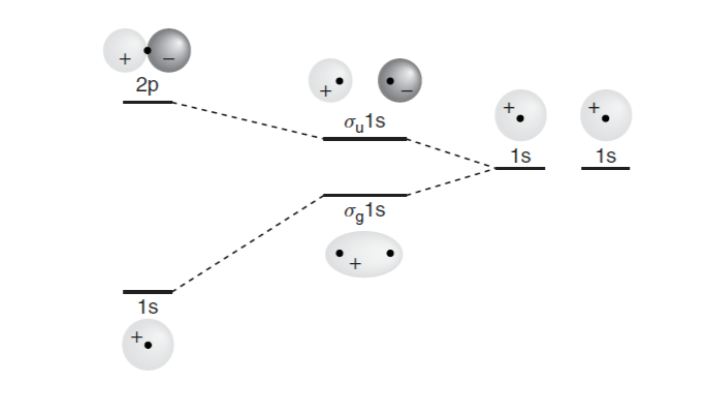
\includegraphics[scale=0.6]{Images3/Distance mol.PNG}
    \caption{Illustration des atomes à distance $R=0$, $R=R_e$ et $R=\infty$}
    \label{fig:Dist_mol}
\end{figure}
On va donc décrire le cheminement des atomes, de l'état dissocié vers la fusion, puis dans l'autre sens.

\subsection{De $R=\infty$ vers $R=R_e$}

Lorsque deux noyaux se rapprochent, un champ électrique apparaît, et le moment angulaire électronique se quantifie sur l'axe intermoléculaire . $L_z$, qui est la projection de L sur cet axe, va donc dépendre de l'orientation de L par rapport aux deux atomes. La figure \ref{fig:quantification de L} représente en a) l'approche d'un atome dans l'état S et d'un atome dans l'état D et en b) le rapprochement de deux atomes dans l'état P. Pour chaque atome, la grande flèche représente L, et les nombres indiqués correspondent aux différentes valeurs de $m_l$. On peut donc, pour chaque combinaison, obtenir différents états, qui seront notés avec la lettre majuscule grecque correspondante (qui dépend de $M_l$), ainsi que d'un signe +/- dans le cas de $\Sigma$, déterminé par la règle de corrélation de Wigner et Witner. De manière générale, on aura plus d'états plus/moins lorsque $L_1+L_2+\sum_il_{i1}+\sum_il_{i2}$ est paire/impaire. Pour rappel, la somme des $l_i$ correspond à la parité de l'état considéré (g ou u). Les différents états moléculaires possibles pour chaque paires d'atomes sont illustrés dans la figure \ref{fig:termes mol}.
\newline
\begin{figure}[tpb]
    \centering
    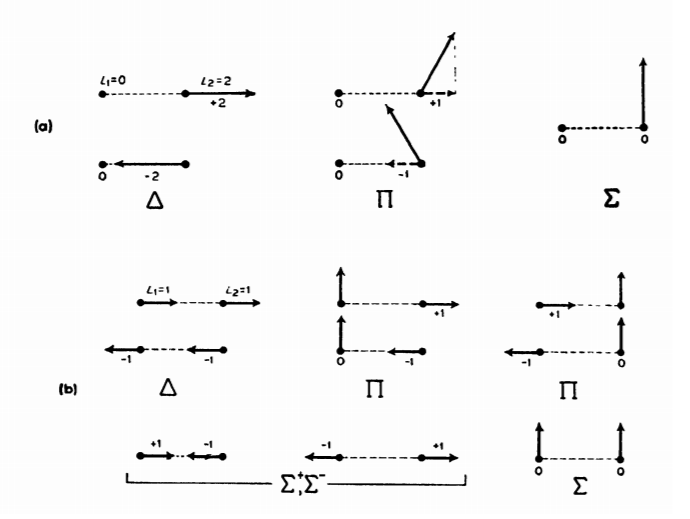
\includegraphics[scale=0.75]{Images3/quantification de L.PNG}
    \caption{Quantification de L suivant l'axe z, pour deux atomes séparés S+D et P+P}
    \label{fig:quantification de L}
\end{figure}
\begin{figure}[tpb]
    \centering
    \includegraphics{Images3/Termes moléculaires.PNG}
    \caption{Détermination des termes moléculaires à partir des termes atomiques}
    \label{fig:termes mol}
\end{figure}
Dans le cas de molécules homonucléaires, comme $H_2$, chaque état est dédoublé, car il existe une version paire et impaire de chacun d'eux, notée toujours u ou g.\newline
Dans les cas où le couplage LS est faible, on peut utiliser les règles de couplage de moment angulaire
classiques pour considérer les multiplicités de spin possibles, qui auront les valeurs suivantes : $\abs{S_1+S_2}$, $\abs{S_1+S_2}-1$, $\abs{S_1+S_2}-2$, ...,$\abs{S_1-S_2}$.
\begin{figure}
    \centering
    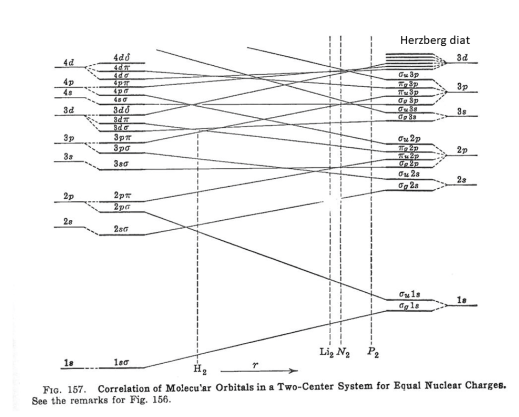
\includegraphics[scale=0.65]{Images3/Corrélation homonucléaire.png}
    \caption{Corrélation des orbitales moléculaires pour des molécules homonucléaires}
\end{figure}
\begin{figure}
    \centering
    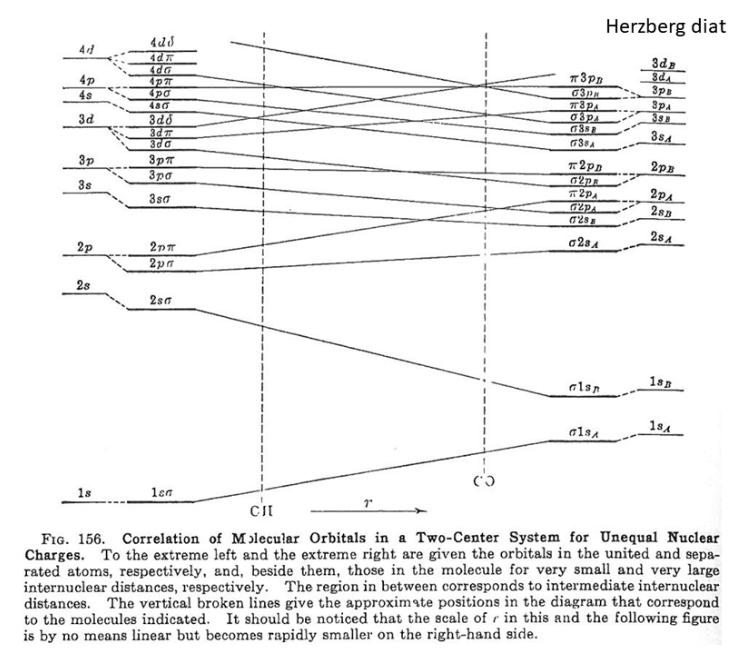
\includegraphics[scale=0.45]{Images3/Corrélation hétéronucléaire.png}
    \caption{Corrélation des orbitales moléculaires pour des molécules hétéronucléaires}
\end{figure}
\clearpage

\subsection{De $R=0$ à $R=R_e$}

Dans ce cadre, on considère que le spin est conservé, et que les valeurs de $M_l$ sont L, L-1, ..., 0. Par exemple, si l'on considère la fission d'un atome de Magnésium en oxyde de Béryllium ou en dicarbone, on aura, en partant d'un état atomique $^3D_g$, des états moléculaires $^3\Delta$, $^3\Pi$ et $^3\Sigma$ \footnote{Le nombre précédant la lettre grecque dans la notation de l'état correspond à 2S+1, avec S le spin total.}. Dans le cas du dicarbone, ces états seront pairs, car les molécules homonucléaires gardent la parité de l'atome fissionné. 

\subsection{Détermination des états moléculaires de l'$O_2$}

\begin{figure}[ht]
    \centering
    \includegraphics[scale=0.6]{Images3/orbitales moléculaires.png}
    \caption{Représentation des orbitales moléculaires pour des molécules diatomiques homonucléaires. En (b) pour les molécules plus légères que $N_2$ ($N_2$ comprise) et en (c) pour les molécules plus lourdes (de $O_2$ à $Ne_2$).}
    \label{fig:orbitales}
\end{figure}
On prendra la molécule de dioxygène ($O_2$) comme exemple pour cette partie.\newline
On sait que la le dioxygène possède 16 électrons, qu'il faut donc répartir sur les orbitales disponibles. Pour cela, il suffit d'utiliser la figure \ref{fig:orbitales} et de remplir les orbitales en partant du bas. Les électrons étant des fermions, on ne peut en mettre que 2 par orbitales (un de spin up et un de spin down). On aura donc la configuration suivante : 
\begin{equation*}
    (1\sigma_g)^2(1\sigma^*_u)^2(2\sigma_g)^2(2\sigma^*_u)^2(3\sigma_g)^2(1\pi_u)^4(1\pi^*_g)^2
\end{equation*}
Comme dans le cas atomique, toutes les couches jusque $(1\pi_u)^4$ sont fermées, et seule la dernière est ouverte. Sur cette dernière couche, on a 4 états possibles pour les électrons, et donc 6 combinaisons pour les deux électrons de la dernière couche, qui sont représentés dans le tableau de la figure \ref{fig:Combinaisons}. Ces électrons sont forcément de type $\pi_g$, avec une valeur de $m_l$ de $\pm1$ (représenté par l'indice +1 ou -1 en dessous du g dans le tableau) et un spin positif ou négatif (une barre surmontant l'état correspond à un spin négatif, et son absence à un spin positif).\newline
\begin{figure}
    \centering
    \includegraphics[scale=0.7]{Images3/Combinaisons électroniques.png}
    \caption{Combinaisons possibles pour les deux électrons de la dernière couche de $O_2$ et valeurs de $M_l$ et $M_s$ correspondantes.}
    \label{fig:Combinaisons}
\end{figure}
On pourra donc avoir un état $^1\Delta_g$ dégénéré en $M_l$ (en bleu), et des états $^3\Sigma_g$ et $^1\Sigma_g$, en fonction des valeurs de $M_s$. On peut ensuite déterminer si les états $\Sigma$ sont + ou -. Pour cela, il faut déterminer la valeur propre de l'opérateur $\sigma_v$. Commençons par l'état $M_l = 0$ et $M_s=1$ :  
\begin{equation*}
    \begin{split}
        \phi(M_l=0, M_s=1) &= \abs{\pi_{g_{+1}}\;\pi_{g_{-1}}}\\
        &= \frac{1}{\sqrt{2}}
        \begin{vmatrix}
            \pi_{g_{+1}}(1) & \pi_{g_{-1}}(1)\\
            \pi_{g_{+1}}(2) & \pi_{g_{-1}}(2)\\
        \end{vmatrix}\\
        &= \frac{1}{\sqrt{2}}(\pi_{g_{+1}}(1)\pi_{g_{-1}}(2)-\pi_{g_{-1}}(1)\pi_{g_{+1}}(2))\\
    \end{split}
\end{equation*}
On peut maintenant appliquer $\sigma_v$ sur cette fonction pour voir la valeur propre associée \footnote{Pour rappel, $\sigma_v$ à pour effet de changer le signe de $m_l$.}: 
\begin{equation*}
    \begin{split}
        \sigma_v\phi &= \frac{1}{\sqrt{2}}(\pi_{g_{-1}}(1)\pi_{g_{+1}}(2)-\pi_{g_{+1}}(1)\pi_{g_{-1}}(2))\\
        &= -\phi
    \end{split}
\end{equation*}
La valeur propre de $\sigma_v$ est donc -1, l'état triplet sigma se note alors : $^3\Sigma_g^-$.\newline
Pour passer à l'état $M_l = 0$ et $M_s = 0$, on va utiliser un opérateur de descente en spin pour les deux électrons sur l'état $M_l = 0$, $M_s = 1$ traité précédemment. Ce qui nous donne : 
\begin{equation*}
    \abs{\overline{\pi}_{g_{+1}}\;\pi_{g_{-1}}} + \abs{\pi_{g_{+1}}\;\overline{\pi}_{g_{-1}}}
\end{equation*}
Comme la base doit être orthogonale, on peut définir la fonction d'onde électronique de l'état singulet sigma : 
\begin{equation*}
    \begin{split}
        \phi =& \abs{\overline{\pi}_{g_{+1}}\;\pi_{g_{-1}}} - \abs{\pi_{g_{+1}}\;\overline{\pi}_{g_{-1}}}\\
        =& \frac{1}{\sqrt{2}}(\overline{\pi}{g_{+1}}(1)\pi_{g_{-1}}(2) - \pi_{g_{-1}}(1)\overline{\pi}_{g_{+1}}(2) - \pi_{g_{+1}}(1)\overline{\pi}_{g_{-1}}(2) + \overline{\pi}_{g_{-1}}(1)\pi_{g_{+1}}(2))
    \end{split}
\end{equation*}
On peut maintenant y appliquer $\sigma_v$ : 
\begin{equation*}
    \begin{split}
        \sigma_v\phi &= \frac{1}{\sqrt{2}}(\overline{\pi}{g_{-1}}(1)\pi_{g_{+1}}(2) - \pi_{g_{+1}}(1)\overline{\pi}_{g_{-1}}(2) - \pi_{g_{-1}}(1)\overline{\pi}_{g_{+1}}(2) + \overline{\pi}_{g_{+1}}(1)\pi_{g_{-1}}(2))\\
        &= \phi
    \end{split}
\end{equation*}
La valeur propre de $\sigma_v$ est donc +1, l'état singulet sigma se note alors : $^1\Sigma_g^+$.\newline
On peut maintenant étudier séparément la partie spatiale et la partie de spin pour les deux fonctions d'ondes, et on remarquera que la partie spatiale de $^3\Sigma_g^-$ est antisymétrique par rapport à la permutation des électrons, alors que la partie de spin est symétrique, et pour l'état $^1\Sigma^+_g$ c'est l'inverse.\newline
Grâce à la règle de Hund, on peut déterminer que l'état fondamental sera l'état $^3\Sigma_g^-$, le premier état excité sera $^1\Delta_g$ et le second sera $^1\Sigma^+_g$.\newline
Le cas de $N_2$ a également été fait en cours, mais le principe est le même.
\begin{figure}
    \centering
    \includegraphics[scale=0.6]{Images3/Table des termes moléculaires.PNG}
    \caption{Table des termes moléculaires possibles en fonction des combinaisons électroniques.}
    \label{fig:termes_mol}
\end{figure}

\section{Spectroscopie de molécules diatomiques}

Les objectifs de cette sections sont de déterminer les règles de sélection, i.e. entre quelles paires de niveaux une transition peut avoir lieu, ainsi que les facteurs dont dépendent la probabilité de transition.\newline
Pour rappel, en physique atomique, une transition radiative (avec absorption ou émission de photon) ne peut advenir que si :
\begin{equation*}
    \mel{\psi'}{\mu}{\psi''} \neq 0
\end{equation*}
Et l'intensité de la transition sera proportionnelle au carré de ce terme.\newline
Dans cette équation, on note $\psi'$ l'état excité, $\psi''$ l'état de départ et $\mu$ le moment dipolaire électrique défini comme suit : 
\begin{equation*}
    \mu = -e\sum\limits_i\Vec{r}_i + Z_1e\Vec{R_1} + Z_2e\Vec{R_2}
\end{equation*}
Le dipôle étant donc séparable en une partie électronique (le premier terme, que l'on peut noter $\mu_{el}$) et une partie nucléaire (les deux derniers termes, notés $\mu_{nucl}$). Il est important de noter que $\mu$ est impair comparativement à l'opération $E^*$ (inversion des coordonnées x, y et z).\newline
Pour évaluer l'interaction entre la lumière et la molécule, il faut projeter le moment dipolaire dans le référentiel du champ électromagnétique oscillant associé à la lumière. En considérant une fonction d'onde dans le cadre de l'approximation de Born-Oppenheimer ($\Psi(r,R) = \phi^{Nu}_m(R)\psi^{el}_m(r;R)$), la condition de transition peut s'écrire :
\begin{equation*}
    \mu_{mk} = \int (\psi^{el}_m\phi^{Nu}_m|\mu^{el} + \mu^{Nu}|\psi^{el}_k\phi^{Nu}_k)d\tau_{el}d\tau_{Nu}
\end{equation*}
Déjà à partir de cette équation, on peut déduire deux règles de sélection. En effet, comme les fonctions de base de spin sont orthonormales, on peut s'attendre à ne pas observer de variation de spin électronique ($\Delta S = 0$) ou nucléaire ($\Delta I =0$). On peut maintenant réécrire cette intégrale en séparant la partie nucléaire et électronique :
\begin{equation*}
    \mu_{mk} = \int \phi^{Nu}_m\left[\int \psi^{el}_m\mu^{el}\psi^{el}_kd\tau_{el} \right]\phi^{Nu}_kd\tau_{Nu} + \int \phi^{Nu}_m\left[\int \psi^{el}_m\psi^{el}_kd\tau_{el} \right]\phi^{Nu}_kd\tau_{Nu}
\end{equation*}
Pour que ces intégrales soient non-nulles, il faut que l'intégrant soit pair, et même totalement symétrique. Comme $\mu$ et ses deux composantes $\mu_{el}$ et $\mu_{Nu}$ sont impairs par rapport à $E^*$, on réalise que la première intégrale implique un changement de parité lors de la transition électronique, et la seconde implique une transition au sein d'un état électronique (spectre de rotation-vibration).

\subsection{Spectres de rotation-vibration}

Reprenons l'intégrale de rotation-vibration : 
\begin{equation*}
    \int \phi^{Nu}_m\left[\int \psi^{el}_m\psi^{el}_kd\tau_{el} \right]\phi^{Nu}_kd\tau_{Nu}
\end{equation*}
Ce terme est bien nul si $m\neq k$ (car les $\psi^{el}_m$ forment une base orthonormée), mais il est également nul dans le cas d'une molécule homonucléaire. En effet, $\mu_{Nu} = Z_1e\Vec{R_1} + Z_2e\Vec{R_2}$, or $Z_1=Z_2$ et $\Vec{R_1}=-\Vec{R_2}$ si les deux atomes sont identiques, $\mu_{Nu}$ est donc nul dans ce cas.\newline
Dans la section \ref{Solutions de l'hamiltonien}, on avait considéré que les problèmes vibrationnels et rotationnels étaient découplés. On peut alors obtenir :
\begin{equation*}
    \psi(r,Q,\theta,\phi) = \psi^{el}_m(r;R)\frac{\psi(Q)}{R}Y_J^M(\theta,\phi)
\end{equation*}
Avec $Q = \sqrt{\mu}(R-R_e)$ (attention, ici $\mu$ est la masse réduite et pas le moment dipolaire), et \footnote{Le développement se trouve à la section \ref{Solutions de l'hamiltonien}}
\begin{equation*}
    \psi_v(Q) = \left[(\frac{\gamma}{\pi})^{\frac{1}{2}}\frac{1}{2^v(v!)} \right]^{\frac{1}{2}}e^{\frac{1}{2}\gamma Q^2}H_v(\gamma^{\frac{1}{2}}Q)
\end{equation*}
On peut maintenant projeter le moment dipolaire moléculaire du référentiel fixé sur la molécule au référentiel dans lequel se propage la lumière : 
\begin{equation*}
    \mu(R) = ||\mu(R)||\sin{(\theta)}\cos{(\phi)}\hat{x} + ||\mu(R)||\sin{(\theta)}\sin{(\phi)}\hat{y} +||\mu(R)||\cos{(\theta)}\hat{z}
\end{equation*}
Pour rappel, l'élément de volume en coordonnées sphériques est : 
\begin{equation*}
    dV = R^2\sin{\theta}dRd\theta d\phi
\end{equation*}
On peut donc calculer la contribution du terme en $\mu^{Nu}_{mk}$ : 
\begin{equation*}
    \begin{split}
        \mu_{mk} &= \int^{\infty}_0\psi_v''(q)\psi_v'(q)\mu^{Nu}(R)dR\\
        &= \int^{2\pi}_0\int^{\pi}_0 Y_J''^M{}''Y_J'^M{}'(||\mu(R)||\sin{(\theta)}\cos{(\phi)}\hat{x} + ||\mu(R)||\sin{(\theta)}\sin{(\phi)}\hat{y} +||\mu(R)||\cos{(\theta)}\hat{z})d\theta d\phi
    \end{split}
\end{equation*}
Cette dernière double intégrale sera notée Ang dans la suite, elle permet d'obtenir les règles de sélection sur le moment angulaire J et sa projection M. Celles-ci sont les suivantes :
\begin{equation*}
    \begin{split}
        \Delta J &= \pm1\\
        \Delta M &= 0 \textrm{ ($\mu_Z$),} \pm1 \textrm{ ($\mu_{X,Y}$)}
    \end{split}
\end{equation*}
L'intégrale suivant R peut être évaluée grâce à un développement de Taylor du moment dipolaire autour de la position d'équilibre :
\begin{equation*}
    \mu^{Nu}(R) = \mu^{Nu}(R_e) + \dv{\mu^{Nu}}{R}\left.\right|_{R_e}(R-R_e) + \frac{1}{2}\dv[2]{\mu^{Nu}}{R}\left.\right|_{R_e}(R-R_e)^2
\end{equation*}
On peut alors écrire : 
\begin{equation*}
    \begin{split}
        \mu_{mk} =& \int^{\infty}_0\psi_v''(q)\psi_v'(q)\mu^{Nu}(R)dRAng\\
         =& \int^{\infty}_0\psi_v''(q)\psi_v'(q)\mu^{Nu}(R_e)dRAng \; \neq 0 \textrm{ Si $v' = v''$}\\
         &+ \dv{\mu^{Nu}}{R}\left.\right|_{R_e}\int^{\infty}_0\psi_v''(q)\psi_v'(q)(R-R_e)(R_e)dRAng \; \neq 0 \textrm{ Si $v' = v''\pm1$}\\
         &+ \frac{1}{2}\dv[2]{\mu^{Nu}}{R}\left.\right|_{R_e}\int^{\infty}_0\psi_v''(q)\psi_v'(q)(R-R_e)^2(R_e)dRAng \; \neq 0 \textrm{ Si $v' = v''\pm2$}\\
         &+ \hdots
    \end{split}
\end{equation*}
Plus le potentiel électronique sera proche du potentiel harmonique plus la série de Taylor convergera rapidement. Le terme principal sera donc celui des rotations pures ($\Delta v = 0$) ou éventuellement des bandes fondamentales ($\Delta v = \pm1$).

\subsection{Transitions électroniques}

Reprenons maintenant le terme de transitions entre états : 
\begin{equation*}
    \int \phi^{Nu}_m\left[\int \psi^{el}_m\mu^{el}\psi^{el}_kd\tau_{el} \right]\phi^{Nu}_kd\tau_{Nu}
\end{equation*}
Définissons : 
\begin{equation*}
    \mu^{el}_{mk} \equiv \int \psi^{el}_m\mu^{el}\psi^{el}_kd\tau_{el}
\end{equation*}
On peut alors décomposer $\phi_m^{Nu}$ en une composante vibrationnelle et rotationnelle :
\begin{equation*}
    \phi_m^{Nu} = \psi_{vm}Y_J^M(\theta,\phi)
\end{equation*}
Si on considère que $\mu^{el}_{mk}$ est indépendant des coordonnées nucléaires (approximation du centroïde), on peut réécrire la première intégrale comme :
\begin{equation*}
    \mu^{el}_{mk} \int \phi^{Nu}_m\phi^{Nu}_kd\tau_{Nu}
\end{equation*}
Où l'intégrale est appelée facteur de Franck-Condon. Avec cette approximation, on aura un transfert de paquet d'onde rovibrationnelle d'un état à un autre, appelé "transition verticale". L'intensité de la transition va dépendre du recouvrement des fonctions d'ondes vibrationnelles associées à deux états électroniques et vibrationnels différents. On peut, après quelques développements, trouver les règles de sélection suivantes : 
\begin{equation*}
    \begin{split}
        \Delta S &= 0\\
        \Delta\Lambda &= 0,\pm1\\
        \Delta J &= 0 \textrm{ Sauf pour $\Sigma-\Sigma$, c'est $\pm1$}\\
        g &\leftrightarrow u \textrm{ pour les molécules homonucléaires}
    \end{split}
\end{equation*}
La propension à avoir des transitions intenses pour $\Delta v = 0$ ou $\Delta v \neq 0$ va être fonction de la différence de géométrie d'équilibre et d'anharmonicité.\newline
On peut voir sur la figure \ref{fig:recouvrement} que pour des géométries de départ et d'arrivée très proches (figure de gauche), la transition la plus intense sera celle de l'état $v'=0$ vers $v''=0$, car le recouvrement entre ces deux états est important. À l'inverse, lorsque les géométries sont différentes, la transition 0-0 est faible, le maximum étant décalé (ici sur la transition 3-0).
\begin{figure}
    \centering
    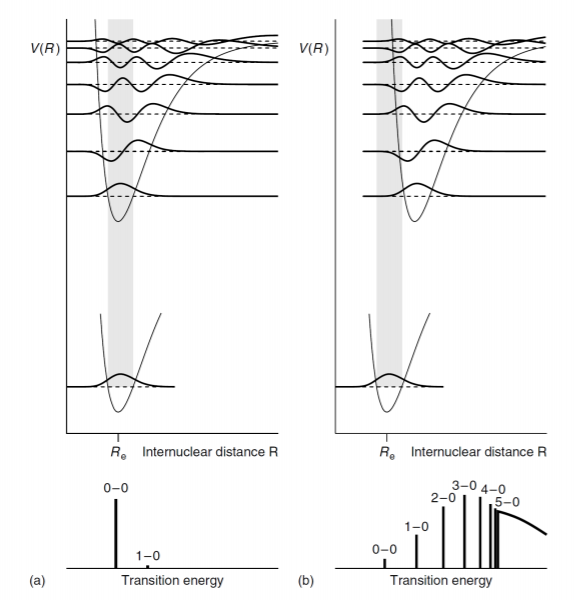
\includegraphics[scale=0.8]{Images3/Recouvrement.PNG}
    \caption{Illustration des variations d'intensité de transitions pour chaque bande vibrationnelle en fonction de la géométrie d'équilibre}
    \label{fig:recouvrement}
\end{figure}
En résumé, l'intensité d'une transition sera donc fonction de  :
\begin{itemize}
    \item $\abs{\mu_{mk}^{el}}^2$\\
    \item Le facteur de Franck Condon\\
    \item Le facteur de Hönl-London : $\abs{\sum\limits_{M''M'}\iint Y_{J''}^{M''}Y_{J'}^{M'}\sin{(\theta)}d\theta d\phi}^2$
\end{itemize}

\subsection{Analyse de spectre}

Le nombre d'onde $\Tilde{\nu}[cm^{-1}]=\frac{1}{\lambda}$ d'une transition électronique peut être estimé comme suit :
\begin{equation*}
    \Tilde{\nu} = [T_{el}'-T_{el}''] + [G_{v'}-G_{v''}] + [F_{J'}-F_{J''}]
\end{equation*}
Avec
\begin{equation*}
    \begin{split}
        G_v &= \omega_e(v+\frac{1}{2})-x_e\omega_e(v+\frac{1}{2})^2 + \hdots\\
        F_J &= B_vJ(J+1) - DJ^2(J+1)^2
    \end{split}
\end{equation*}
En phase gazeuse on peut mesurer des transitions rovibrationnelles isolées et on définit une branche P quand $\Delta J =-1$ et une branche R quand $\Delta J =+1$. On peut donc calculer les nombres d'ondes associés à ces deux branches en posant $J' = J''+1$ pour une branche R et $J' = J'' - 1$ pour une branche P. On obtient alors les expressions suivantes en négligeant la distorsion centrifuge :
\begin{equation*}
    \begin{split}
        \Tilde{\nu_R} &= \Tilde{\nu_0} + 2B_{v'} + (3B_{v'}-B_{v''})J + (B_{v'}-B_{v''})J^2\\
        \Tilde{\nu_P} &= \Tilde{\nu_0} - (B_{v'}+B_{v''})J + (B_{v'}-B_{v''})J^2
    \end{split}
\end{equation*}
Où $\Tilde{\nu_0}$ est définit comme l'origine de bande, et peut être une différence d'énergie vibrationnelle ou vibronique (électronique, vibrationnel et rotationnel couplés).\newline
Par ce type d’étude on obtient des informations sur la dynamique du système (par le profil des transitions), sur la concentration (aire sous la courbe de la transition), une information sur l’identité chimique, la pression, la température, le couplage de moment angulaire et dans le cas de transitions électroniques on peut établir si il y a une variation de géométrie d’équilibre entre les deux états électroniques considérés.





\clearpage